\chapter{Key Points}
\myTop{This chapter describes the key points of our program.
The key points are central functionality from the \hdesk[]. that are included are the complex and medium functions from chapter \ref{cap:classesevents}.
These are chosen because they are central functions to the entire system.
%We want to search for problems to avoid clients committing similar problems and to search the database for a specific problem according to the system definition in section \ref{sec:systemdefinition}.
%We have also chosen that our system should balance the workload between staff members in order to provide more efficient solving as we state in our system definition.
}
\section{Problem Prioritization}
\label{sec:problem_priority}
%When a problem is added to the system the priority of the problems is calculated based on the tags attached to the problem.
The priority of a problem is used in the staffs worklist, where all problems are sorted by priority, however all problems with deadlines are shown first on the list.
The division of the worklist is made to create a better overview.
If a problem with an approved deadline is overdue, the priority will go up to the maximum priority, which in turn will make the problem appear on the top of the list.

\begin{comment}
The priority of a problem is based on two factors:

%When assigning multiple problems to a staff member, they will appear as a list. 
%Due to the human nature, we might pick a specific order of solving the problems in, which does not necessarily take priority, deadlines and such into account. 
%Therefore, the order of which the problems appear in the staff members work list, is important.
%We have defined two elements which define a problems importance, and therefore its placement in the list of problems. 
%These two elements are:

\begin{itemize}
	\item Whether or not a deadline is approved
	\item The priority of the tags attached to the problem
\end{itemize}
\end{comment}

The worklist should be sorted because some problems are more important then others and should be solved prior to lesser important problems. 

When a staff member is assigned to a problem, he should read the new problem and approve the problems deadline if it is reasonable. 

%The list is ordered by priority of the problem, however problems with approved deadlines will always appear on top of the list regardless of their or other problems priority. 
%This splits the list into two parts. Above, priority-sorted problems with approved deadlines, and below priority-sorted problems with or without not approved deadlines. 

An example of a worklist can be seen in figure \ref{fig:worklist}.
\section{Problem Search}
\label{sec:search}
Our application needs to be able to search for problems.
The method for this specific purpose is simply called \me{Search} and is 
This search is based on tags.
It should find an amount of problems which match the specified tags and order them by number of tags matching.
%It will find an amount of problems which match the specified tags and order them by number of tags matching.
The amount of problems this function will find is depending on a specified number know as ``Minimum number of problems'', which determines when the function should stop searching for more problems.

The input for this function is:

\begin{itemize}
	\item Selected tags
	\item Problems to search among
	\item All tags
	\item Minimum number of problems to find
\end{itemize}

The \me{Search} function is called with the parameters above. It calls an \me{InternalSearch} function -- which is private -- with the same parameters and a compare delegate which determines how the problems should be sorted.
The \me{InternalSearch} function is described in subsection \ref{sub:searchTags} and \ref{sub:noTags}.
Subsection \ref{sub:orderSolved} describes the \me{SearchSolvedFirst} function, which takes into account whether or not a problem is solved, when ordering the list of problems to return.
It does so by calling the \me{InternalSearch} function with another compare delegate.

\subsection{Search for Problems by Tags}
\label{sub:searchTags}
\begin{lstlisting}[style=sourceCode, caption=\myCaption{The while loop which finds and sorts problems matching the input tags}, label=src:search, numbers=left, numberstyle=\footnotesize,float=hp]
...
while (result.Count < listMinSize && noOfTagsToRemove < tags.Count)(*\label{search:whileStart}*)
{
	tempResult = new List<Problem>();
	tagsToRemove = new List<int>();
	for (int i = 0; i < noOfTagsToRemove; i++)(*\label{search:forStart}*)
	{
		tagsToRemove.Add(i);
	}(*\label{search:forEnd}*)
	try(*\label{search:tryStart}*)
	{
		List<Tag> currentSearch = tags.RemoveCurrent(tagsToRemove);
		while (true)(*\label{search:innerWhileStart}*)
		{
			temp = allProblems.ToList();
			foreach (Tag tag in currentSearch)(*\label{search:foreachStart}*)
			{
				temp = temp.Where(x => x.Tags.Contains(allTags.FirstOrDefault(y => y.Id == tag.Id))).ToList();
			}(*\label{search:foreachEnd}*)
			tempResult.AddRangeNoDuplicates(temp.ToList());
			currentSearch = tags.RemoveNext(ref tagsToRemove);(*\label{search:removeNext}*)
		}(*\label{search:innerWhileEnd}*)
	}
	catch (NotSupportedException)
	{
		noOfTagsToRemove++;
		tempResult.Sort(compare);
		result.AddRangeNoDuplicates(tempResult.ToList());
	}
}(*\label{search:whileEnd}*)
...
\end{lstlisting}

The most important part of the \me{InternalSearch} function is the while loop shown in code snippet \ref{src:search}.
Generally, this loop finds problems which match the tags specified in the input to the function and orders them with the problems with the most amount of matching tags in the beginning of the result list.
The while loop beginning in line \ref{search:whileStart} will continue to run as long as there has not been found enough problems to suffice the minimum number of problems input and there still is at least one tag to search for.
If there still is not enough problems another part of the search function will take care of this.
This part is described in subsection \ref{sub:noTags}.

The function will increase the number of tags to remove from the tag list which was input to the function every time an iteration ends in the outer while loop; lines \ref{search:whileStart}-\ref{search:whileEnd}.
In the first iteration no tags are removed, this means that the function will find every problem which has every tag which is being search for and put these in the beginning of the result list.
Furthermore the function sorts the problems each step by the least amount of tags. Because the less tags a problem have which are not searched for, the more likely it is that the given problem matches the search.
For example if a search is run for the tags ``Computer'' and ``Harddisk'', the problems only containing these tags will be listed first and if a problem contains the tags ``Computer'', ``Harddisk'', ``Database'', and ``Connection'' it will be listed further down on the result list because it has unrelated tags attached to it.
%See a more detailed example of a run of the search function in appendix \ref{something}\fixme{Tilf\o j dette eksempel eller fjern denne linje}.

The inner while loop spanning the lines \ref{search:innerWhileStart}-\ref{search:innerWhileEnd} iterates over the tags to remove, this does not have any effect when no tags are to be removed.
However if the function gets the tags ``Computer'' and ``Harddisk'' as input, we first want to find every problem with both tags, then find every problem with the ``Computer'' tag, and finally find every tag with the ``Harddisk'' tag.
The order of the last two is not important because they are sorted in a single list, which is then inserted into the result list.
The \me{RemoveNext} function called in line \ref{search:removeNext} is responsible removing the tags which are not to be search for in the in the next iteration of the inner while loop in lines \ref{search:innerWhileStart}-\ref{search:innerWhileEnd}.
It will throw a \cl{NotSupportedException} when it has removed every combination of tags, which will break the inner while loop and add the problems found in the current search to the result list, which will be returned to the call site later.
The function \me{AddRangeNoDuplicates}, is used instead of the in-build \me{AddRange} function, because otherwise one problem could be added several times, which is not wanted.
One problem should only appear one time in the list returned from this function, because it would simply not make sense in relation to the minimum number of problems, since a single problem would be counted several times towards finding enough problems.
Furthermore the client seaching for problems should not have the same problem appear on his/her list more than once.
Therefore at some point in our code we would have to filter out the duplicates, we chose to do it here, because it is the earliest step in finding problems in our database.
If we were to filter the duplicates out another place, the search function could potentially return a list containing a single problem several times, which when filtered only yields a single problem and thereby rendering the minimum number of problems nearly useless.

The for-each loop in the lines \ref{search:foreachStart}-\ref{search:foreachEnd} finds all the problems match the current search.
The current search is the tags being input to the function without the tags to be removed.
The for-each loop removes every problem not containing a specific tag in each iteration, until every tag in the current search is covered.

The initialization of the tags to remove is done in the for loop in the lines \ref{search:forStart}-\ref{search:forEnd}.
It sets the first $x$ tags to be removed where $x$ is the current number tags to remove.
This means that if e.g. three tags should be removed it will initially be the first, second and third tag, which are removed.

\subsection{No Tags to Remove}
\label{sub:noTags}
If there has not been found enough problems to suffice the minimum number of problems during the search in tags the function will start to look for problems with no tags at all, then problems with one tag etc.
This part of the function will start by finding every problem with no tags and add them to the result list, and then every problem with a single tag is found and added.
Here the problems are also added using the \me{AddRangeNoDuplicates} applying the same reasoning as above.
This part of the function will continue to run until enough problems are found or it is about to search for more tags then there is in the ``All tags'' input.
This means that it can actually return less problems than minimum number of problems if it cannot find any more, but at this point it has examine every problem, this means that it will actually return every problem in the ``Problems to search among'' sorted.

\subsection{Order by Solved}
\label{sub:orderSolved}
In some cases we want to order the problems by whether or not the problems are solved.
E.g. we want to show the solved problems first to clients who are categorizing a problem, which might already exist.
The reason for this is that the client should be presented with problems with a solution first, in hope that the client can use a solution and does not need to subscribe to a problem or add a new one.

This \me{Search} method makes use of the \me{InternalSearch} method but with a different compare input to the \me{Sort} function.
This compare function sorts first by whether or not a problem is solved, then by the least number of tags.
\section{Balance Workload}
Whenever a staff is removed from a department or has marked a problem as solved, 
it becomes necessary to balance the workload of each staff member in the department, since we do not want the staff members to be overloaded with problems. 

To balance the workload, each staffs workload must be calculated. 
The workload of a staff is defined by the amount of time estimated that each problem on his workload takes to be solved. 
The workload is calculated by the \me{GetWorkload} method.

The time a problem takes to be solved is estimated by the average time consumption of the tags connected to the problem. 
This is calculated by the \me{CalculateTimeConsumption} method.

The \me{BalanceWorkload} method works by finding the staff in the department with the minimum workload and the staff with the maximum workload. Then it moves the highest priority problems from the maximum staff to the minimum. 
It keeps reassigning problems until the minimum staff has a higher or equal workload than the maximum staff. If it is higher the problem is reassigned back. 
All this is iterated once per staff minus one in the department. 
E.g. if there are two staffs it is ran once, if there is three it yields two etc. 
The pseudo code is displayed in code snippet \ref{lst:balanceWorkload}.

The primary concern of the algorithm is to distribute the problems so each staff has as balanced workload as possible.

 
%This balance is based on the time of all the individual staff members problems are approximated to take.
%This balance is based on the time approximated that all problems on his workload consumes. 
%							den tid alle de individuelle staff medlemmers problemer er approximeret til at tage, tilsammen.
%Balancen er baseret p\aa{} den tid alle staff problemer er approximeret til at tage tilsammen. 


We also wanted the algorithm to take the individual priority of the problems into account. 
This algorithm makes sure that the high priority problems will be distributed. 
If the priority was unrelevant the algorithm would take the problem with lowest time consume, since this would give the most balanced workload. 
An example of the algorithm is shown on figure \ref{fig:balanceWorkloadDiagram}. 

%There is one weakness though and that is if a staff has a highly time consuming problem with low priority. Then he will be left with only that problem. Assuming it is as time consuming as all the other problems. 


\begin{figure}
	\centering
		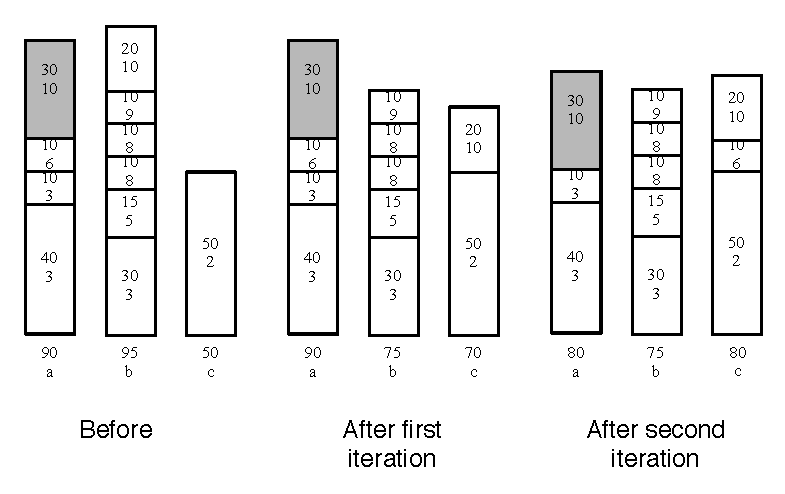
\includegraphics[scale=0.8]{input/implementation/key_points/balanceWorkloadDiagram.pdf}
	\morscaption{A diagram of the balance workload method. Each collumn represents a staffs workload. Each box is a problem. The upper number is the estimated time consumed of that problem. The lower is the priority. The problem colored dark grey is not reassignable.  There are tree staffs a, b, and c. The problems that will be moved is colored light grey. }
	\label{fig:balanceWorkloadDiagram}
\end{figure}


\begin{lstlisting}[style=sourceCode, caption=\myCaption{A code snippet of the balance workload method. The presented code is within a for loop running each for every staff minus one}, label=lst:balanceWorkload]
var max = Persons.FirstOrDefault(y => 	
		y.GetWorkload() == Persons.Max(x => 
		x.GetWorkload()));                  

var min = Persons.FirstOrDefault(y => 
		y.GetWorkload() == Persons.Min(x => 
		x.GetWorkload()));
    
max.Worklist.ToList().Sort(Problem.GetComparer());             
while(true)
{
    var problemToBeMoved = max.Worklist.FirstOrDefault(y => 
		y.Reassignable == true && 
		y.HasBeen == false && 
		y.SolvedAtTime == null);
                   
    if (problemToBeMoved == null)     break; 
    problemToBeMoved.HasBeen = true;
    problemToBeMoved.AssignedTo = min;
    
    if (min.Workload > max.Workload)
    {
    	problemToBeMoved.AssignedTo = max;
    	break;
    }
    else if (min.Workload == max.Workload)
    {
		break;
    }
} 
\end{lstlisting}




\subsection{eta}
\label{}


Get workload kalder ETA
\section{Tag Time Management}
\label{sec:managetagtimes}

The \me{ManageTagTimes} method updates the statistics held by each tag whener a staff member marks a problem as solved and submits the number of hourse he/she used solving it. The \me{ManageTagTimes} method is a property of the \cl{Problem} class in the model.
The idea behind it is simply to increment the \verb+SolvedProblems+ and \verb+TimeConsumed+ properties of each tag. The method is shown in code snippet \ref{lst:managetagtimes}.

\begin{lstlisting}[style=sourceCode, caption=\myCaption{The ManageTagTimes method}, label=lst:managetagtimes]
public void ManageTagTimes(double StaffTimeSpentInput)
{
    string StaffTimeSpent = StaffTimeSpentInput.ToString();
    string[] split = StaffTimeSpent.Split(".".ToCharArray());
    
    int HoursUsed = Int32.Parse(split[0]);
    int MinutesUsed = 0;

    try
    {
        MinutesUsed = (int)(0.6*(double.Parse(split[1]))) + (HoursUsed*60);
    }
    catch
    {
        MinutesUsed = HoursUsed*60;
    }

    foreach (var tag in Tags)
    {
        if (tag.SolvedProblems == null)
            tag.SolvedProblems = 0;
        
        tag.SolvedProblems++;

        if (tag.TimeConsumed == null)
            tag.TimeConsumed = 0;

        tag.TimeConsumed = tag.TimeConsumed + MinutesUsed;
    }
}
\end{lstlisting}
\sec{Estimated Time Consumption}
\label{sec:estimated_time_consumption}

The \me{CalculateEstimatedTimeConsumption()} function -- which is a method in \cl{Problem} class -- estimates how much time is needed to solve the specific problem, under the assumption that there only exists this single problem on the assigned staff members queue. The idea is to sum up all the \verb+AverageTimeSpent+ property as well as all the count the number of tags, and lastly calculate the average time for all the tags. See code snippet \ref{lst:estimatedtimeconsumption}.

\begin{lstlisting}[style=sourceCode, caption=\myCaption{The ManageTagTimes method}, label=lst:estimatedtimeconsumption]
public TimeSpan EstimatedTimeConsumption
{
    get
    {
        return CalculateEstimatedTimeConsumption();
    }
}

private TimeSpan CalculateEstimatedTimeConsumption()
{
    int NumberOfTags = 0;
    decimal? ProblemTime = 0;
    int Minutes = 0;
    int Hours = 0;
    int Days = 0;

    decimal? average = 0;

    foreach (Tag tag in Tags)
    {
        if (tag.AverageTimeSpent != null)
        {
            ProblemTime = ProblemTime + tag.AverageTimeSpent;
        }
        NumberOfTags++;
    }

    if (NumberOfTags == 0)
    {
        average = 10;
    }
    else
    {
        average = ProblemTime / NumberOfTags;
    }

    Hours = (int)average % 60;
    Minutes = (int)average - (Hours*60);
    Days = Hours % 24;
    Hours = Hours - (Days * 24);

    return new TimeSpan(Days, Hours, Minutes, 0);
}
\end{lstlisting}
\section{Expected Time Of Completion}
\label{sec:expected_time_of_completion}



\begin{lstlisting}[style=sourceCode, caption=\myCaption{The CalculateETA method}, label=lst:calculateeta,float=h]
private DateTime CalculateETA()
{
    DateTime DateTime = DateTime.Now;
    foreach (Problem problem in AssignedTo.SortedWorklist)
    {
        DateTime = DateTime.Add(Estimated¨TimeConsumption);
        if (problem.Id == Id)
            break;
    }
    return DateTime;
}
\end{lstlisting}

The \me{CalculateETA} method -- which is a method in \cl{Problem} class -- estimates time when a specific problem will be solved, based on all the problems in the staff members worklist. The method is shown in code snippet \ref{lst:calculateeta}

\section{Get Sorted List}
\label{sec:getsortedlist}



\begin{lstlisting}[style=sourceCode, caption=\myCaption{The ManageTagTimes method}, label=lst:getsortedlist,float=hp]
private List<Problem> GetSortedList()
{
    List<Problem> problemList = Worklist.ToList().Where(x => x.SolvedAtTime == null && x.IsDeadlineApproved == true).ToList();

    List<Problem> problemWithoutDeadline = Worklist.ToList().Where(x => x.SolvedAtTime == null && (x.IsDeadlineApproved == false || x.IsDeadlineApproved == null)).ToList();


    problemList.Sort(Problem.GetComparer());

    problemWithoutDeadline.Sort(Problem.GetComparer());

    problemList.AddRange(problemWithoutDeadline);

    return problemList;
}
\end{lstlisting}

The \me{GetSortedList} method -- shown in code snippet \ref{lst:getsortedlist} -- purpose is to sort the staff members worklist as defined in section \ref{sec:problem_priority}. 


\section{Reset Person Password}
\label{sec:resetpersonpassword}

\begin{lstlisting}[style=sourceCode, caption=\myCaption{The \me{PassMail} method}, label=lst:passmail,float=hp]
[Authorize(Roles = HoplaHelpdesk.Models.Constants.AdminRoleName)]
public ActionResult PassMail(int id)
{
    //Getting name from person user
    var person = db.PersonSet.FirstOrDefault(x => x.Id == id);
    String user = person.Name.ToString();
    try
    {
        //Used for testing
        string msg = HttpUtility.HtmlEncode("Person.PassMail, User = " + user);
            
        //Preparing mail
        MailMessage mail = new MailMessage();
        //Setting up a smtp client
        SmtpClient SmtpServer = new SmtpClient("smtp.gmail.com");
        //Adding a from mailaddress
        mail.From = new MailAddress("helps305a@gmail.com");
        //Adding user to maillist, by using getmail function.
        mail.To.Add(SQLf.GetEmail(user));

        //Adding a subject and a message for the mail
        mail.Subject = "Hopla Helpdesk: Your password has been changed!";
        mail.Body = "Username: " + user + "\nPassword: " + SQLf.ResetPassword(user) + "\n\nDo not reply to this email.\n--\nKind Regards\nHopla Helpdesk - Staff Team";

        //Config the Smtpserver details
        SmtpServer.Port = 587;
        SmtpServer.Credentials = new System.Net.NetworkCredential("helps305a", "trekant01");
        SmtpServer.EnableSsl = true;

        //Sending mail
        SmtpServer.Send(mail);

        //Adding view if mail was success
        ViewData["Success"] = "The users password was reset to a random value and emailed to the user.";
        ViewData["View"] = "Index";
        return View("Success");
    }
    catch
    {
        //An error view will be added if an error occurred
        ViewData["Error"] = "The password cannot be resetted, " + user + " don't have a mail";
        ViewData["View"] = "Index";
        return View("Error");
    }
}
\end{lstlisting}


\begin{lstlisting}[style=sourceCode, caption=\myCaption{The ResetPassword(String user) method}, label=lst:resetpersonpassword,float=hp]
public static String ResetPassword(String user)
{   
    //Connection
    SqlConnection cn = new SqlConnection();
    cn.ConnectionString = connString;
    //Preparing SqlCommand
    SqlCommand password;
    SqlCommand userId;

    //SqlCommand to find UserId
    userId = new SqlCommand("SELECT UserId FROM aspnet_Users WHERE (UserName = '" + user + "')", cn);
    
    //Executing the SqlCommand
    cn.Open();
    String userA = userId.ExecuteScalar().ToString();
    password = new SqlCommand("SELECT Password FROM aspnet_Membership WHERE (UserId = '" + userA + "')", cn);
    String passA = password.ExecuteScalar().ToString();
    //Converting Application into a String
    cn.Close();

    String[] passarray =
    {
        "a","b","c","d","e","f","g","h","j", "i" ,"k",
        "l","m","n","o","p","q","r","s","t","u",
        "w","x","y","z","A","B","C","D","E","F",
        "G","H","I","J","K","L","M","N","O","P","Q",
        "R","S","T","U","V","W","X","Y","Z",
        "0","1","2","3","4","5","6","7","8","9"
    };

    String setPass = "";
    //Preparing a two randoms, one for password length and one for picking a char from passarray.
    Random RandomNumber = new Random();
    Random RandomPass = new Random();
    int x = RandomNumber.Next(10,25);
    //Putting the passowrd together
    for (int i = 0; i < x; i++)
    {
        int y = RandomPass.Next(passarray.Length);
        setPass += passarray[y].ToString();
    }
    //Finding the user
    MembershipUser u = Membership.GetUser(user);
    //Generating a new password for the user
    String np = u.ResetPassword();
    //Changing the password for the user by using the the resetted password as old password
    u.ChangePassword(np, setPass);
    return setPass;
}
\end{lstlisting}

The purpose of the \me{PassMail} method -- seen in code snippet \ref{lst:passmail} which is part of the \cl{PersonController} controller -- is to reset a user's password to a new random value, and e-mail it to the user.
Although not a key feature, the \me{PassMail} method implements the functionality which sends a user an e-mail, which we consider a key feature since notifying a user is important.
The \me{PassMail} method utilizes the \me{ResetPassword} method -- seen in code snippet \ref{lst:resetpersonpassword} -- which actually generates the new passwords, and updates the database.

\newpage
\section{Get statistics}
\label{sec:getstatistics}

The \cl{StatisticsController} controller -- seen in code snippet \ref{lst:getstatistics} -- calculates the statistics, by utilizing the \me{AverageTimePerProblem()} method -- seen in code snippet \ref{lst:averagetimeperproblem} --  which utilizes the \me{AverageTimePerProblem()} method as well as the \me{AverageTimePerProblemLastWeek()} methods, which both are wrappers to the \me{AverageTime(string method)} method. All three is shown in code snippet \ref{lst:averagetime}.\\
The purpose is to view statistics 

\begin{lstlisting}[style=sourceCode, caption=\myCaption{The StatisticsController controller}, label=lst:getstatistics]
[Authorize(Roles = Constants.AdminRoleName)]
public class StatisticsController : Controller
{
    hoplaEntities db = new hoplaEntities();
    public ActionResult Index()
    {
        var departments = db.DepartmentSet.ToList();
        int TotalTime = 0;
        int TotalTimeLastWeek = 0;
        int problems = 0;
        foreach(var dep in departments){
           TotalTimeLastWeek = (int)dep.AverageTimePerProblem().TotalMinutes;
           TotalTime = (int)dep.AverageTimePerProblem().TotalMinutes;
           problems++;
        }

        var viewModel = new StatisticViewModel()
        {
            AverageLastWeek = new TimeSpan(0,TotalTimeLastWeek/problems,0),
            AverageAllTime = new TimeSpan(0,TotalTime/problems,0),
            Departments = departments
            
        };
        return View(viewModel);
    }
}
\end{lstlisting}


\begin{lstlisting}[style=sourceCode, caption=\myCaption{The AverageTimePerProblem(string method) method -- which is found in the \cl{Department} class -- together with its wrappers.}, label=lst:averagetimeperproblem]
public TimeSpan AverageTimePerProblem()
{
    return AverageTimePerProblem(null);

}

public TimeSpan AverageTimePerProblemLastWeek()
{
    return AverageTimePerProblem("LastWeek");
}

private TimeSpan AverageTimePerProblem(string method)
{
    int people = 0;
    int totalTime = 0;
    foreach (var person in Persons)
    {
        people++;
        if (method == "LastWeek")
            totalTime = (int)person.AverageTimePerProblemLastWeek().TotalMinutes;
         else 
            totalTime = (int)person.AverageTimePerProblem().TotalMinutes;
    }
    if (people == 0)
        return new TimeSpan();
    else
        return new TimeSpan(0, totalTime / people, 0);
}
\end{lstlisting}

\begin{lstlisting}[style=sourceCode, caption=\myCaption{The AverageTime(string method) method -- which is found in the \cl{Person} class -- together with its wrapper.}, label=lst:averagetime]
public TimeSpan AverageTimePerProblem()
{
    return AverageTime("PerProblem");
}

public TimeSpan AverageTimePerProblemLastWeek()
{
    return AverageTime("LastWeek");
}


private TimeSpan AverageTime(string method)
{
    int totalTime = 0;
    int problems = 0;
      IEnumerable<Problem> worklist = null;
      if (method == "LastWeek")
      {
          var lastWeek = DateTime.Now;
          var aWeek = new TimeSpan(7,0, 0, 0);
          lastWeek = lastWeek.Subtract(aWeek);
          worklist = Worklist.Where(x => x.SolvedAtTime > lastWeek);
      }
      else
      {
          worklist = Worklist.Where(x => x.SolvedAtTime != null);
      }

    foreach(var problem in worklist)
    {
        problems++;
        totalTime = totalTime + (int)((TimeSpan)(problem.SolvedAtTime - problem.Added_date)).TotalMinutes;
    }
    if (problems == 0)
        return new TimeSpan();
    else 
        return new TimeSpan(0, totalTime / problems,0);
}
\end{lstlisting}




\myTail{The key points presented in this chapter are all functions with medium or complex complexity.}